\documentclass[aspectratio=169,10pt]{beamer}
\usepackage[utf8]{inputenc}
\usepackage[ngerman]{babel}
\usepackage{csquotes}
\usepackage{graphicx}
\usepackage{booktabs}
\usepackage{hyperref}
\usepackage{siunitx}
\usepackage{array}

% --- Literaturverwaltung mit biblatex ---
% Stil kann bei Bedarf geändert werden (z. B. numeric, authoryear, apa, ieee)
\usepackage[
  backend=biber,
  style=apa,
  sorting=nyt,
  giveninits=true,
  doi=true,
  isbn=false,
  url=true
]{biblatex}
% APA-Sprachmapping fr deutsche Silbentrennung/Bezeichnungen
\DeclareLanguageMapping{ngerman}{ngerman-apa}
\addbibresource{references.bib}

\usetheme{HM} % our custom theme

% Define custom colors:

% 1) Change the primary colour (hex HTML model):
% \sethmprimarycolor[HTML]{0077CC}

% 2) Set example block title/body colours (title, body):
% \sethmexampleblockcolors[HTML]{00AA66}{F0FFF0}

% 3) Set alert block title/body colours (title, body):
% \sethmalertblockcolors[HTML]{FF7700}{FFF4E6}

% Frametitlet spacing (defaults in theme; override below if needed):
% \sethmframetitletop{4mm} % top spacing (uncomment to change)
% \sethmframetitleleft{6mm} % left spacing (defaults to same as top)

% --- Meta ---
\title{Titel der Präsentation}
\subtitle{Optionaler Untertitel oder Slogan}
\author{Vorname Nachname}
\institute{Organisation oder Unternehmen \\ Abteilung oder Fakultät}
\date{\today}

% Footer text (appears centered in the footline)
\sethmfooter{© Autorenteam – Fakultät BW}

% If your logo has a different filename, set it here:
% \sethmlogo{hm_logo.pdf}

% Optional: separate footer logo (falls back to \sethmlogo if not set)
% To use: uncomment and set your file name
% \sethmfooterlogo{hm_footer_logo.png}

% Optional: table of contents style: numbers | bullets | none (default: numbers)
% \sethmtocstyle{bullets}

% \sethmfootnoteoffset{-10mm}

\begin{document}

\begin{frame}[plain]
  \titlepage
\end{frame}

\begin{frame}{Inhalt}
  \tableofcontents
\end{frame}

\section{Einführung}
\begin{frame}{Einführung}
\begin{itemize}
  \item Stellen Sie hier die wichtigsten Punkte Ihrer Präsentation vor.
  \item Verwenden Sie kurze, prägnante Aussagen und ergänzen Sie sie ggf. um Stichworte.
  \item Betonen Sie Schlüssel- und Fachwörter mit \textbf{fetter Schrift}.
\end{itemize}
\end{frame}

\section{Beispielblöcke}
\begin{frame}{Beispielblöcke}
\begin{block}{Hinweis}
  Neutrale graue Kästen für strukturierte Inhalte.
\end{block}
\begin{exampleblock}{Beispiel}
  Praxisbeispiel – kurze, klare Aussage.
\end{exampleblock}
\end{frame}

\section{Zweispaltiges Layout}
\begin{frame}{Zweispaltiges Layout}
\begin{columns}[T] % [T] für Top-Alignment
  \begin{column}{0.48\textwidth}
    \textbf{Linke Spalte}
    \begin{itemize}
      \item Für Vergleiche geeignet
      \item Text und Aufzählungen
      \item Strukturierte Argumente
    \end{itemize}
  \end{column}
  \hfill
  \begin{column}{0.48\textwidth}
    \textbf{Rechte Spalte}
    \begin{itemize}
      \item Gegenüberstellung
      \item Alternative Ansätze
      \item Pro und Contra
    \end{itemize}
  \end{column}
\end{columns}
\end{frame}

\section{Bilder}
\begin{frame}{Einzelnes Bild mit Beschreibung}
\begin{figure}
  \centering
  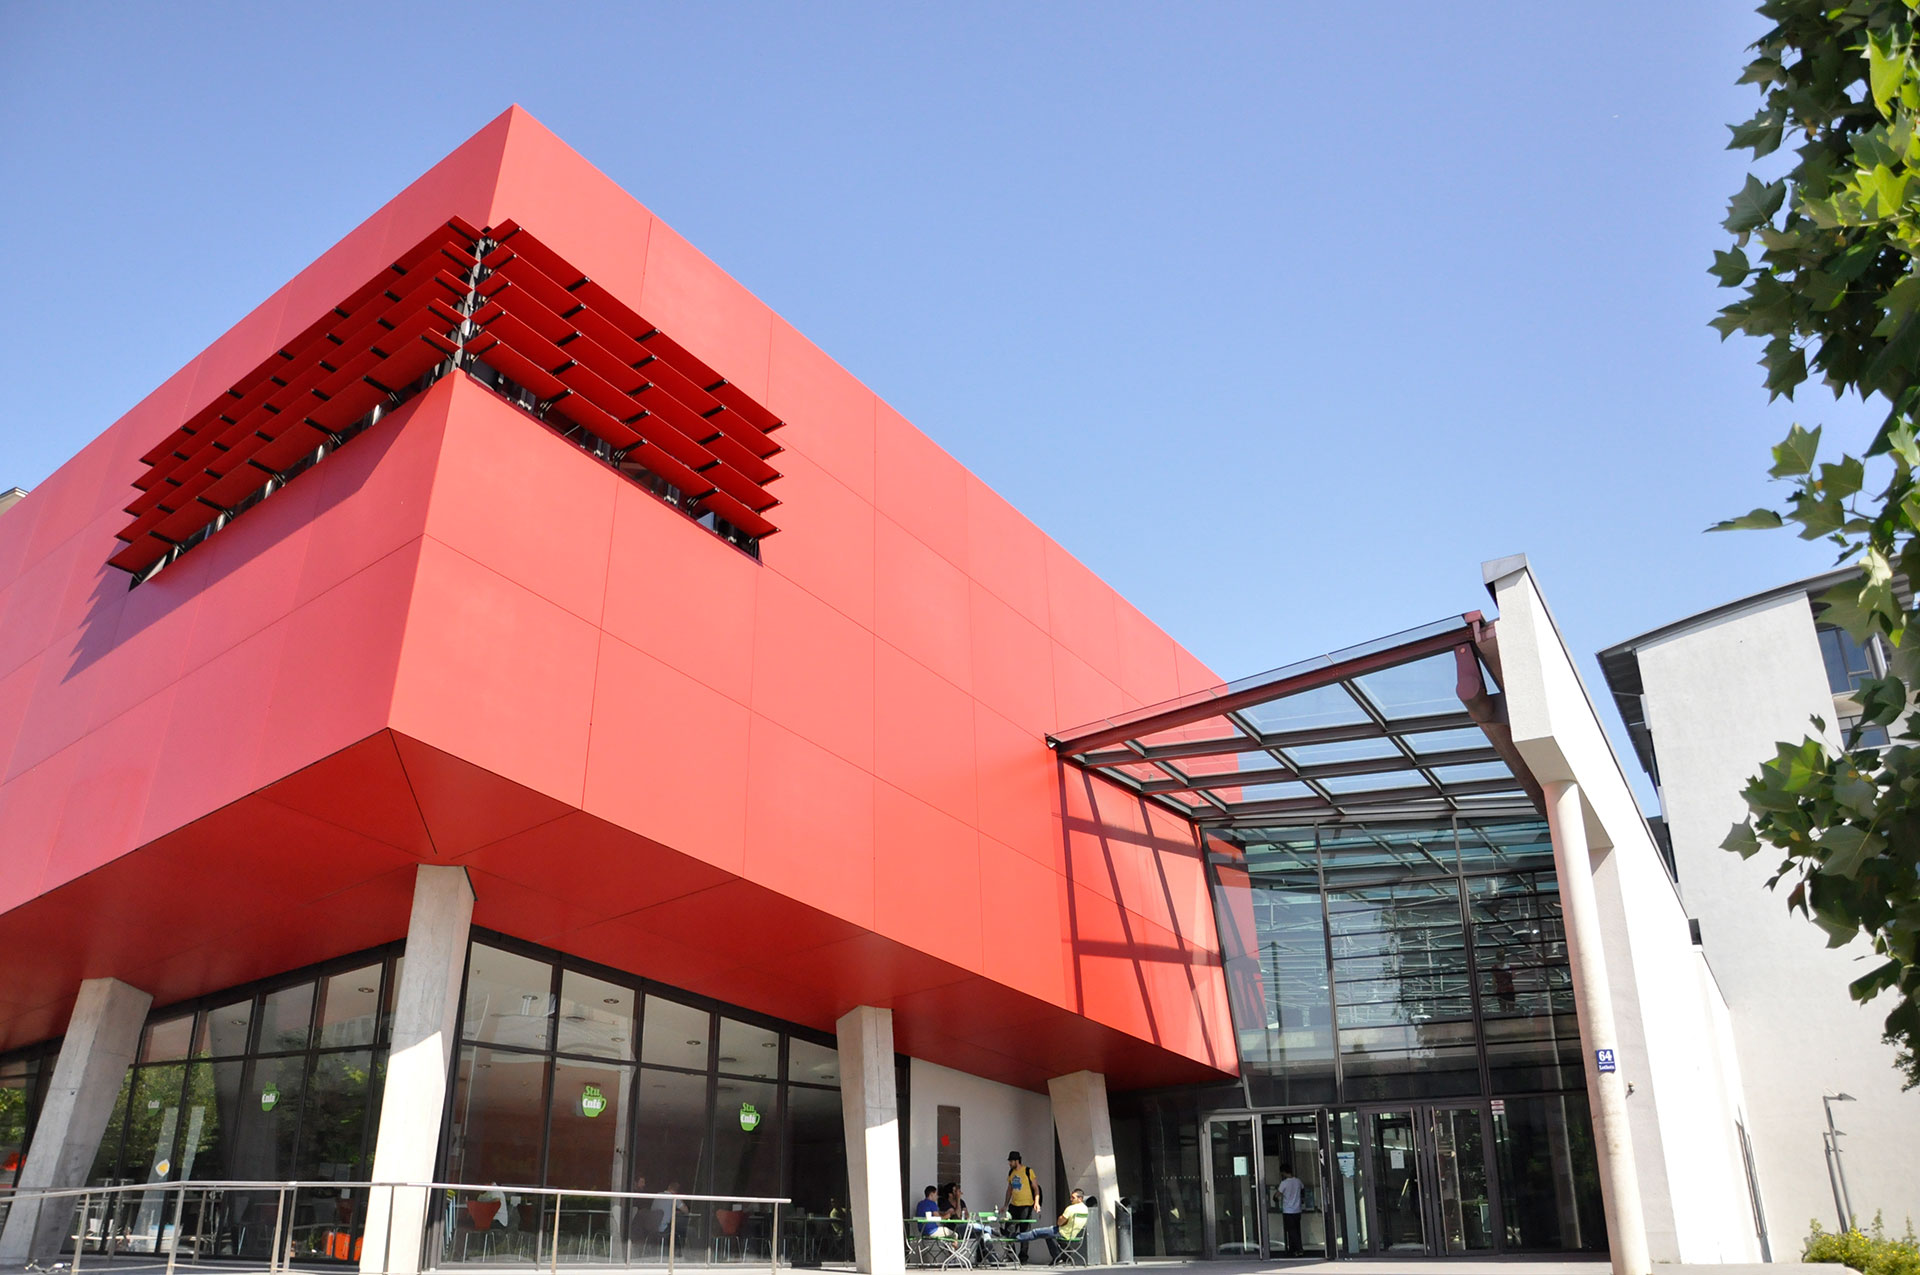
\includegraphics[width=0.6\textwidth]{assets/dm_roter_wuerfel_ben_steinig.jpg}
  \caption{Ein roter Würfel – ideal für Symbolik und visuelle Metaphern}
\end{figure}
\end{frame}

\begin{frame}{Bild und Text nebeneinander}
\begin{columns}[c]
  \begin{column}{0.5\textwidth}
    \begin{itemize}
      \item Kombinieren Sie Bild und Text
      \item Ideal für Erklärungen
      \item Visuelle Unterstützung
      \item Platzsparend und übersichtlich
    \end{itemize}
  \end{column}
  \begin{column}{0.45\textwidth}
    \begin{figure}
      \centering
      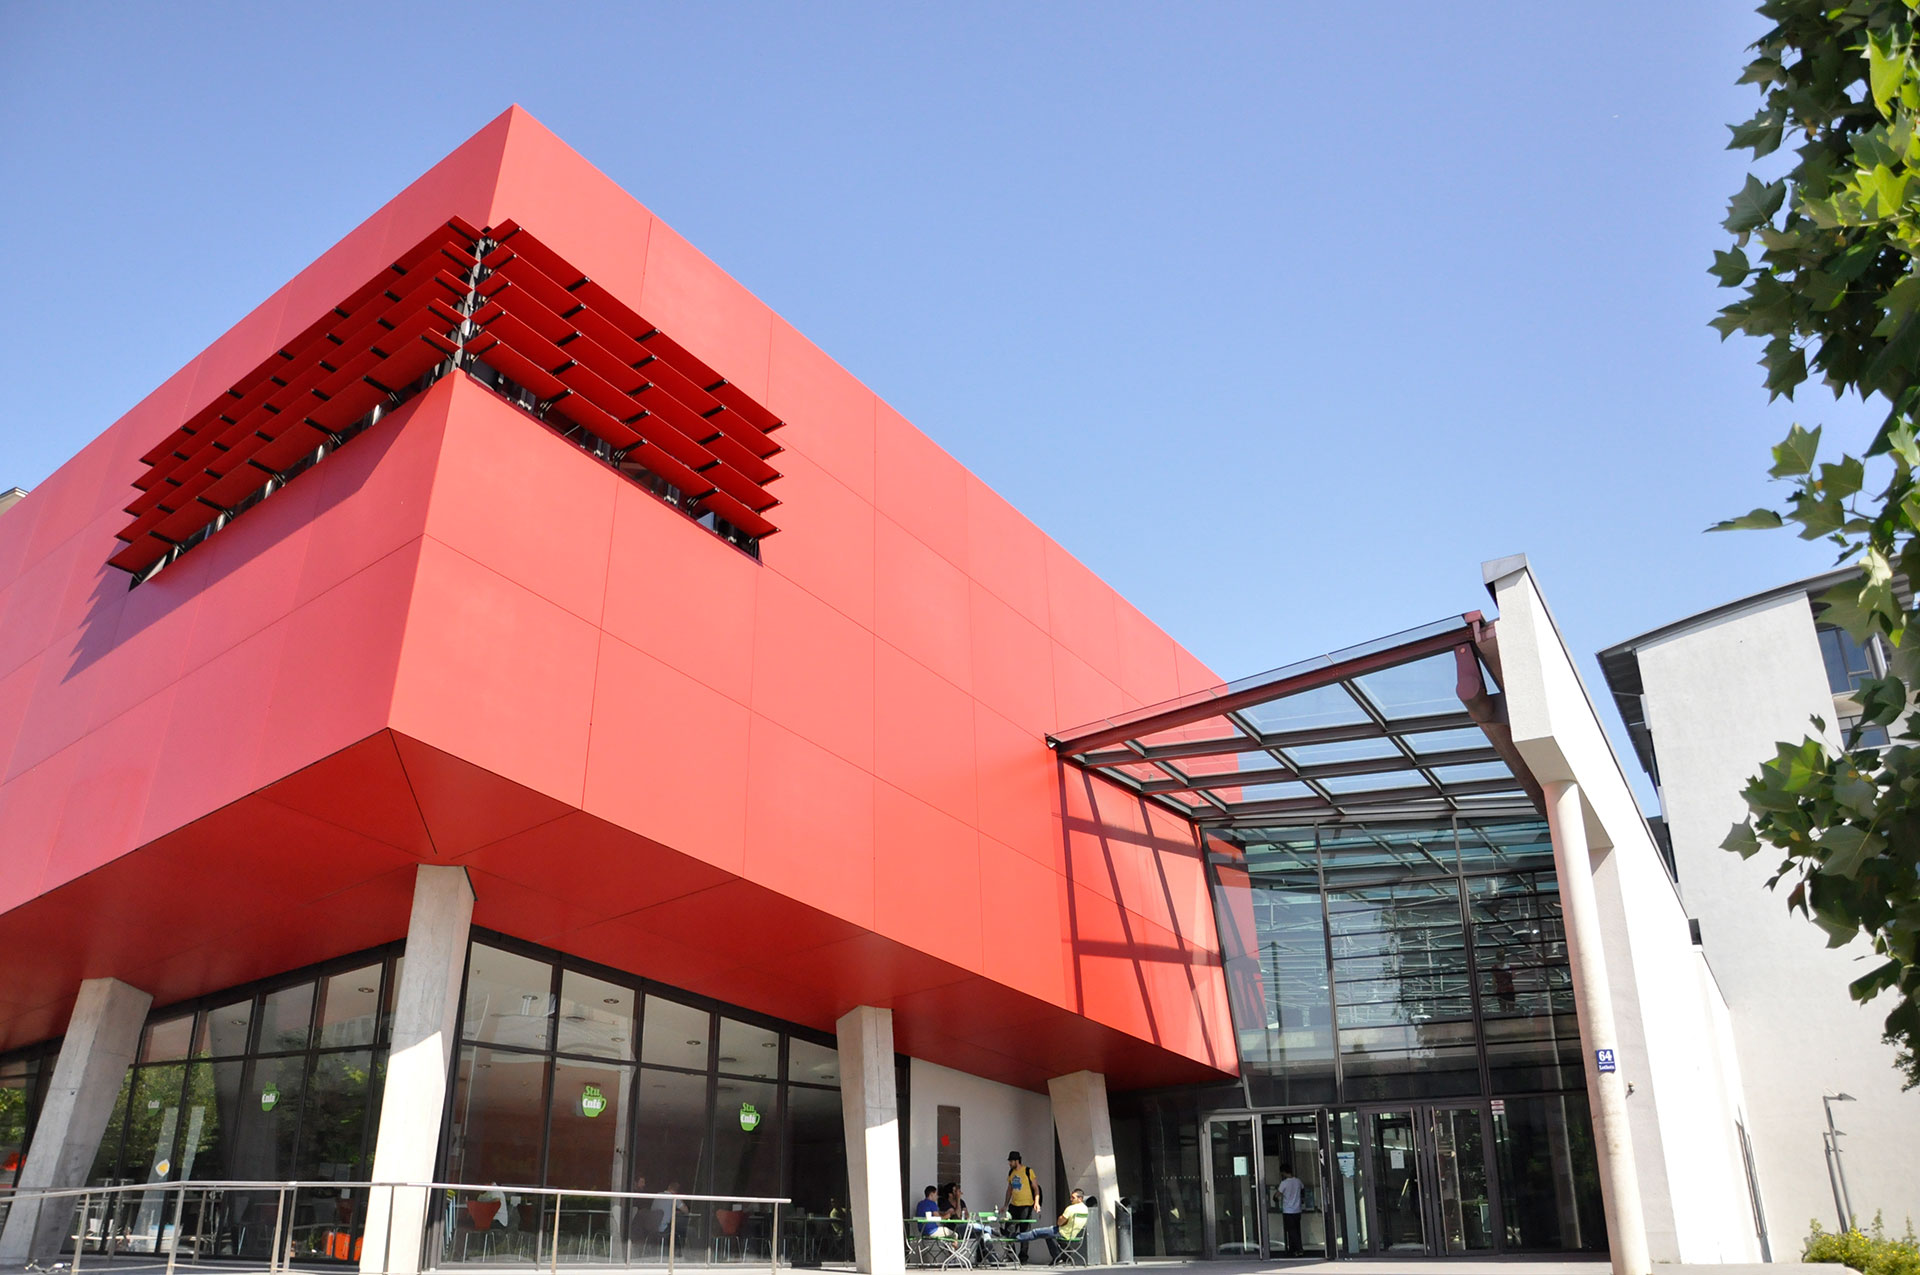
\includegraphics[width=\textwidth]{assets/dm_roter_wuerfel_ben_steinig.jpg}
      \caption{Roter Würfel}
    \end{figure}
  \end{column}
\end{columns}
\end{frame}

\begin{frame}{Zwei Bilder nebeneinander}
\begin{columns}[c]
  \begin{column}{0.48\textwidth}
    \begin{figure}
      \centering
      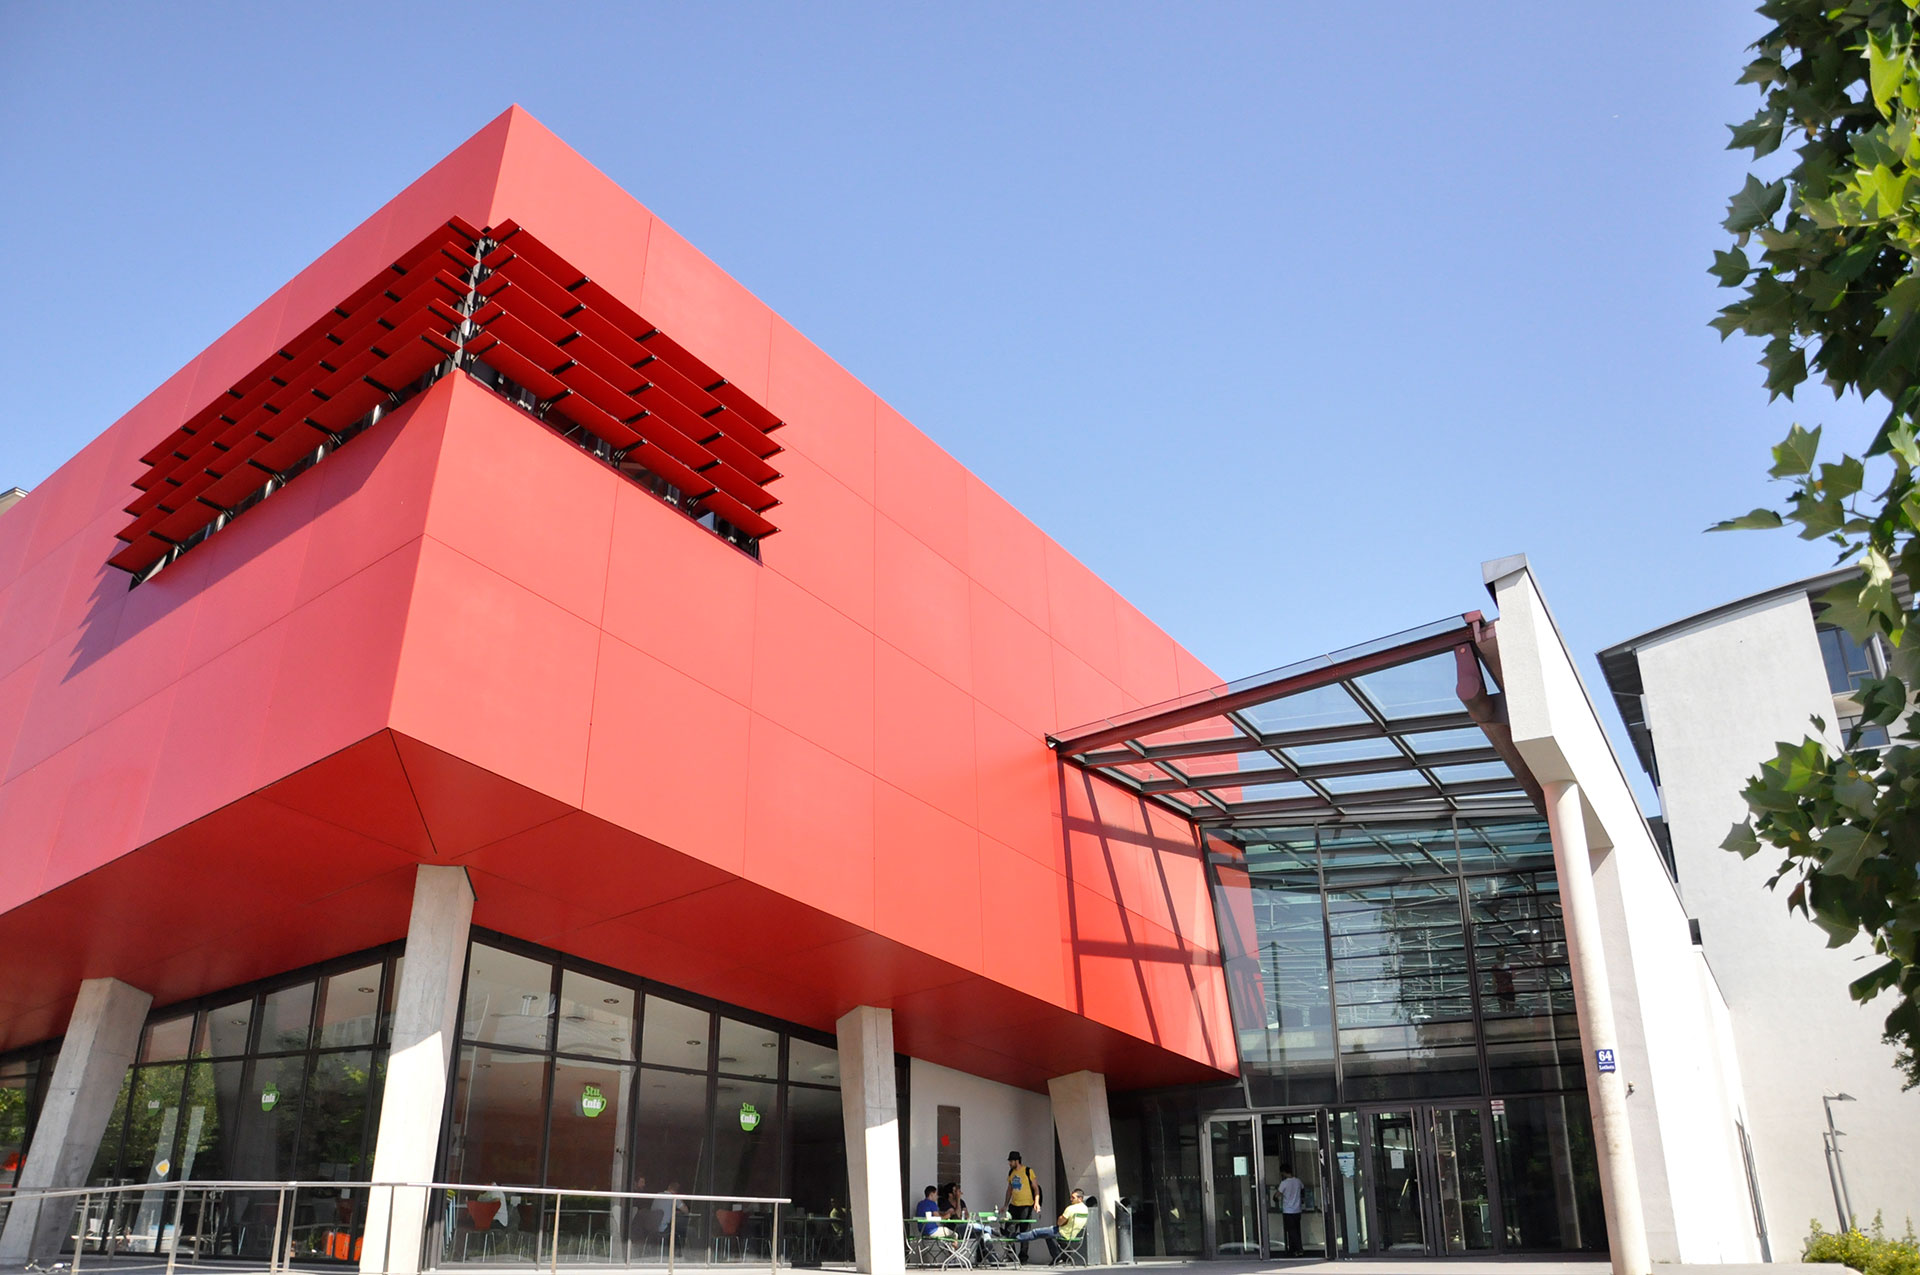
\includegraphics[width=\textwidth]{assets/dm_roter_wuerfel_ben_steinig.jpg}
      \caption{Vorher: Ausgangssituation}
    \end{figure}
  \end{column}
  \hfill
  \begin{column}{0.48\textwidth}
    \begin{figure}
      \centering
      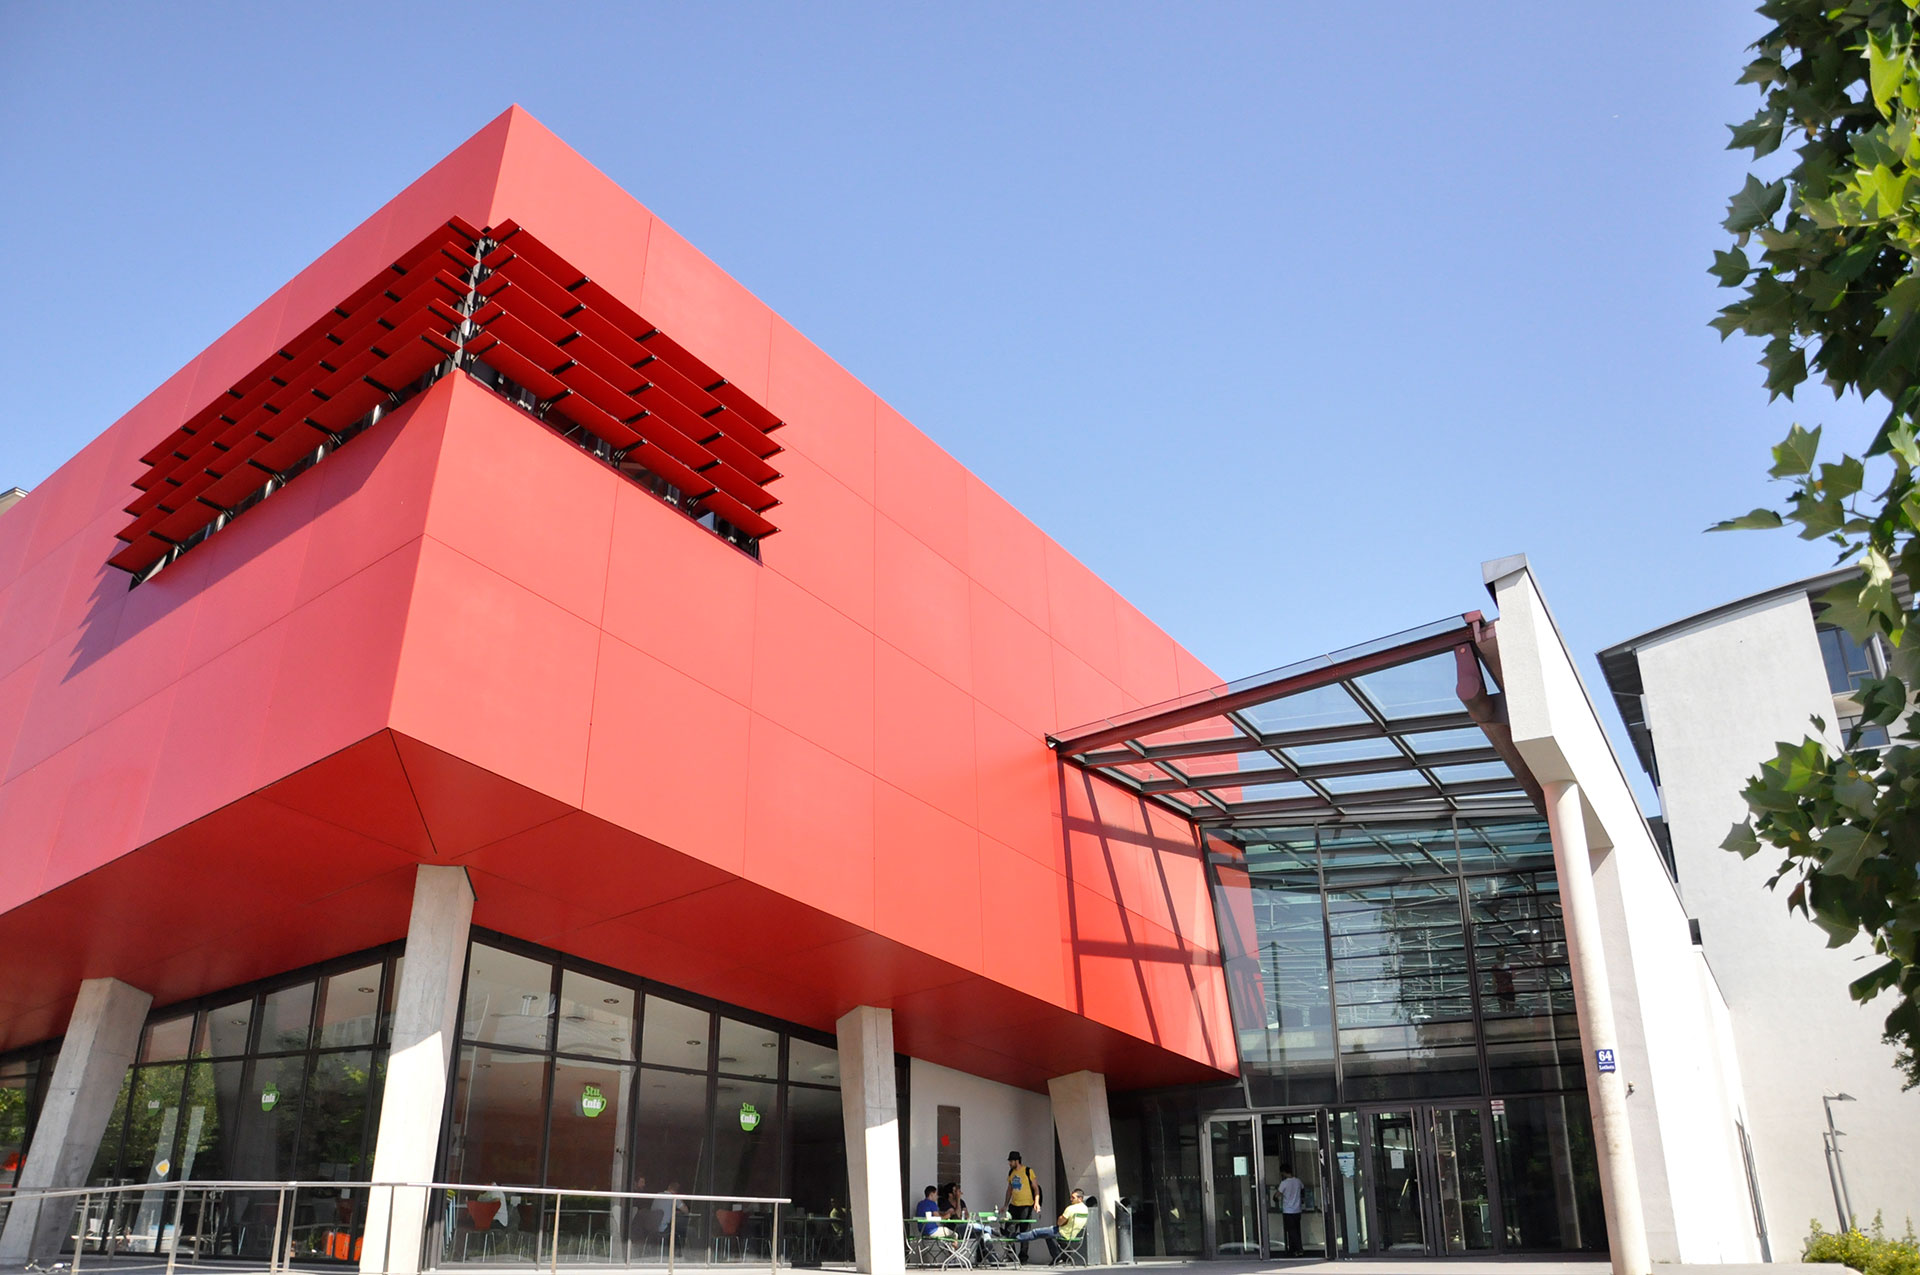
\includegraphics[width=\textwidth]{assets/dm_roter_wuerfel_ben_steinig.jpg}
      \caption{Nachher: Optimierter Zustand}
    \end{figure}
  \end{column}
\end{columns}
\end{frame}

\begin{frame}{Großes Vollbild}
\begin{figure}
  \centering
  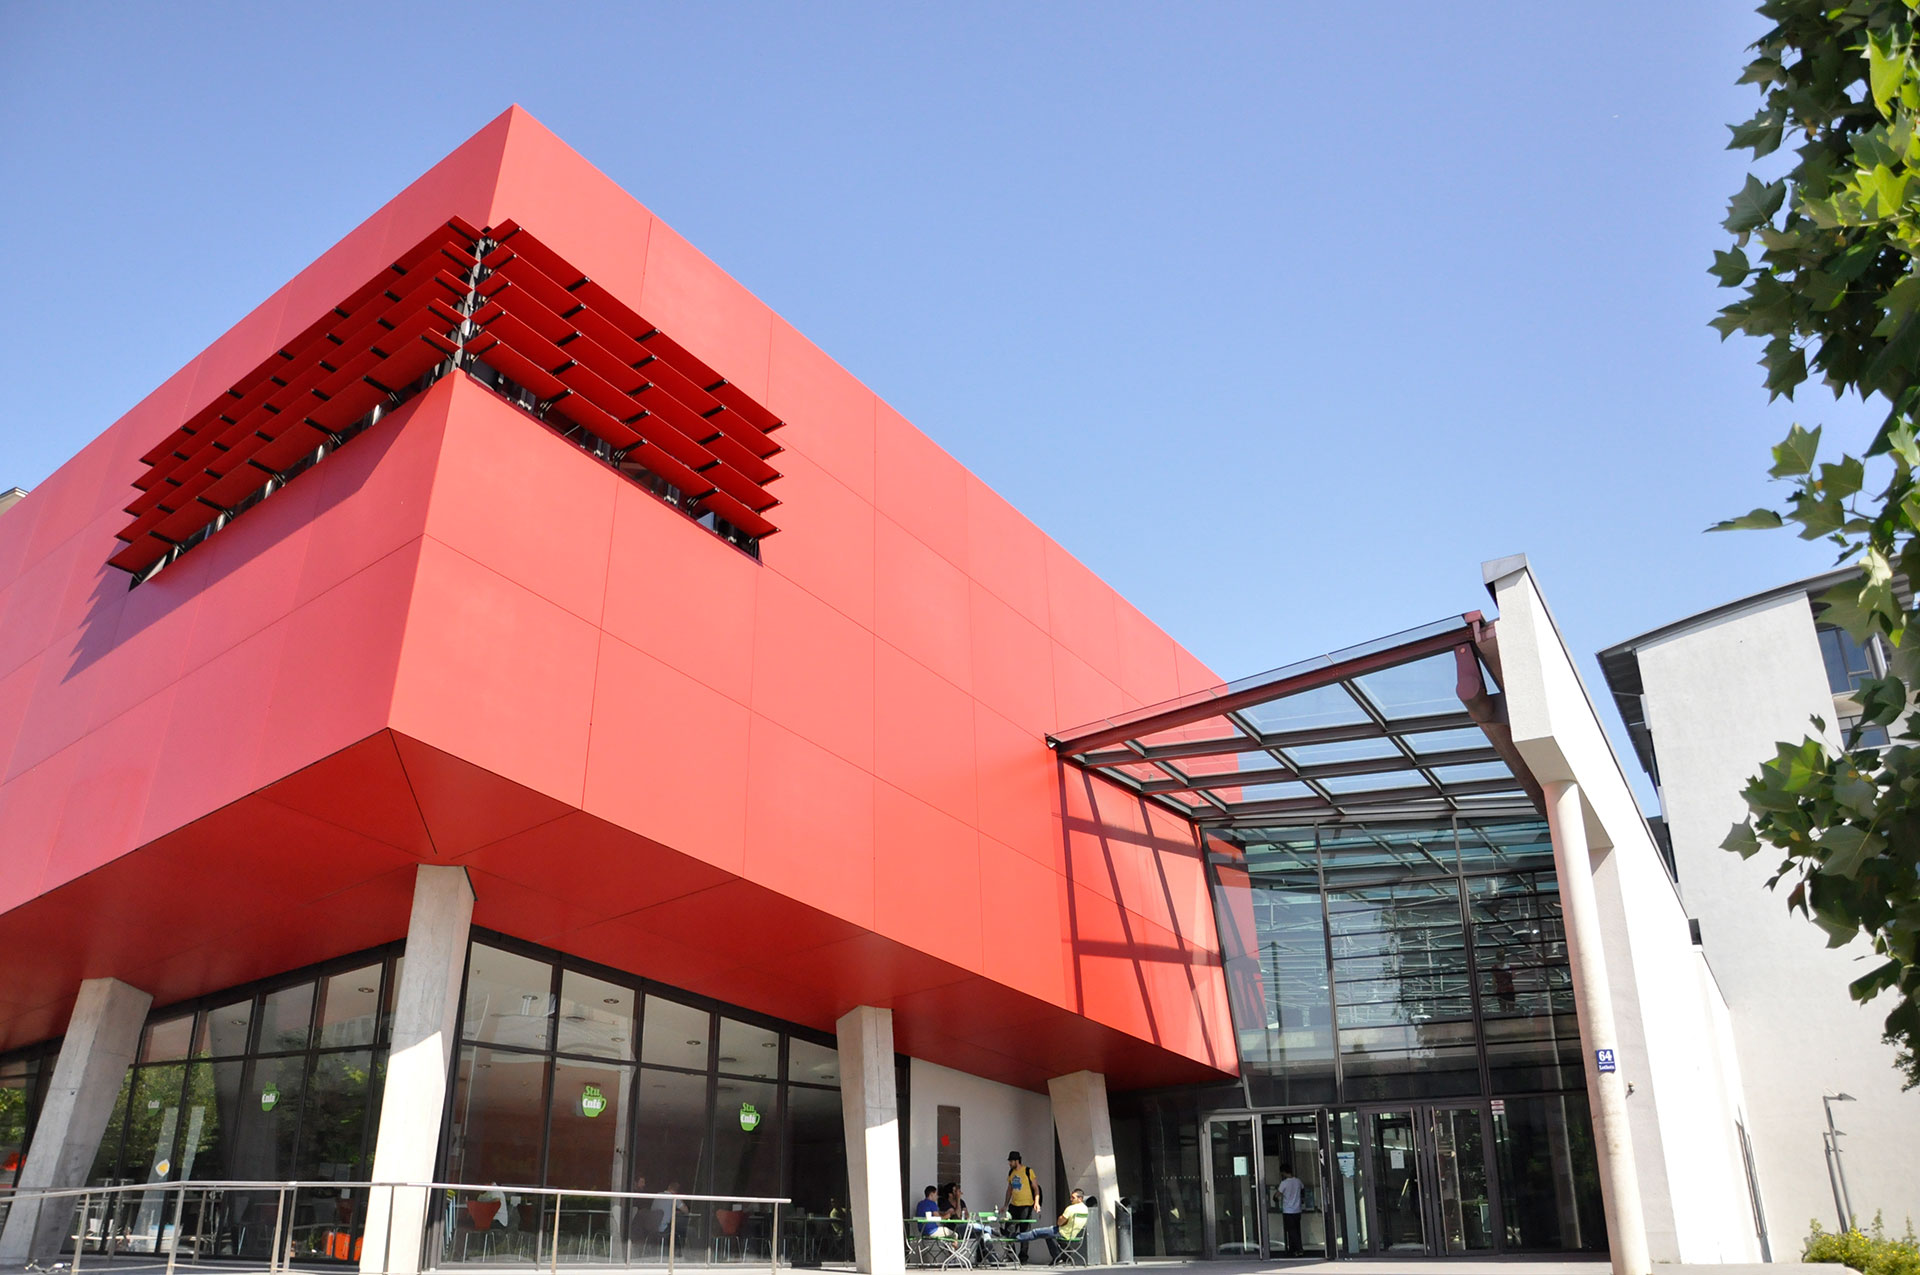
\includegraphics[width=0.9\textwidth,height=0.75\textheight,keepaspectratio]{assets/dm_roter_wuerfel_ben_steinig.jpg}
  \caption{Maximale Bildgröße für starke visuelle Wirkung}
\end{figure}
\end{frame}

\section{Tabellen}
\begin{frame}{Tabelle mit Daten}
\begin{table}
  \centering
  \caption{Übersicht wichtiger Kennzahlen}
  \begin{tabular}{lcc}
    \toprule
    \textbf{Kategorie} & \textbf{2024} & \textbf{2025} \\
    \midrule
    Umsatz (Mio. €) & 45,2 & 52,8 \\
    Wachstum (\%) & 8,5 & 16,8 \\
    Marktanteil (\%) & 12,3 & 14,7 \\
    \bottomrule
  \end{tabular}
\end{table}
\end{frame}

\section{Zitate und Hervorhebungen}
\begin{frame}{Zitat}
\begin{quote}
  \large
  „Ein aussagekräftiges Zitat kann eine Präsentation bereichern und wichtige Botschaften unterstreichen."
\end{quote}
\vspace{0.5cm}
\begin{flushright}
  --- Autor oder Quelle
\end{flushright}
\end{frame}

\begin{frame}{Wichtige Aussage hervorheben}
\begin{center}
  \vspace{1cm}
  {\Huge \textcolor{HMRed}{\textbf{75\%}}}
  
  \vspace{0.5cm}
  {\Large Steigerung der Effizienz}
  
  \vspace{0.5cm}
  durch Optimierung der Prozesse
\end{center}
\end{frame}

\section{Listen und Strukturen}
\begin{frame}{Nummerierte Liste}
\textbf{Schritt-für-Schritt Anleitung:}
\begin{enumerate}
  \item Analyse der Ausgangssituation
  \item Definition der Ziele und Anforderungen
  \item Entwicklung eines Lösungskonzepts
  \item Implementation und Testing
  \item Roll-out und Dokumentation
\end{enumerate}
\end{frame}

\section{Fu\ss{}noten}
\begin{frame}{Fu\ss{}noten-Beispiel}
Ein kurzer Satz mit einer Fu\ss{}note zur Quelle\footnote{Vgl. Beispielstudie 2025, Kap. 3.}. \\
Zus\"atzlich kann eine zweite Anmerkung folgen\footnote{Weitere Details: Stand: \today.}.

\vspace{0.5\baselineskip}
\begin{itemize}
  \item Punkt mit kurzer Erkl\"arung
  \item Langerer Punkt, der \textit{ggf. umbricht} und trotzdem eine saubere
  Platzierung der Fu\ss{}noten oberhalb der Seitenzahl zeigt
\end{itemize}
\end{frame}

\begin{frame}{Verschachtelte Listen}
% Example: show default look. To change markers only for this frame we use a group
% so global templates are not affected.
% The theme now provides sensible defaults for nested item markers (see
% `beamerthemeHM.sty`). If you want to override markers only on this frame,
% uncomment the \begingroup block below and adjust the templates.

%\begingroup
%  % Local marker overrides for demonstration (frame-local)
%  \setbeamertemplate{itemize item}[circle]
%  \setbeamertemplate{itemize subitem}[triangle]
%  \setbeamertemplate{itemize subsubitem}{\raisebox{0.12ex}{\scriptsize$\rightarrow$}}
  \begin{itemize}
    \item \textbf{Hauptpunkt 1}
      \begin{itemize}
        \item Unterpunkt A
        \item Unterpunkt B
          \begin{itemize}
            \item Detaillierter Punkt
          \end{itemize}
      \end{itemize}
    \item \textbf{Hauptpunkt 2}
      \begin{itemize}
        \item Unterpunkt C mit weiteren Details
        \item Unterpunkt D
      \end{itemize}
    \item \textbf{Hauptpunkt 3}
  \end{itemize}
% \endgroup
\end{frame}

\section{Mehrspaltige Inhalte}
\begin{frame}{Drei Spalten}
\begin{columns}[T]
  \begin{column}{0.3\textwidth}
    \centering
    \textbf{\textcolor{HMRed}{Phase 1}}
    
    \vspace{0.3cm}
    Planung und Konzeption
  \end{column}
  \begin{column}{0.3\textwidth}
    \centering
    \textbf{\textcolor{HMRed}{Phase 2}}
    
    \vspace{0.3cm}
    Umsetzung und Testing
  \end{column}
  \begin{column}{0.3\textwidth}
    \centering
    \textbf{\textcolor{HMRed}{Phase 3}}
    
    \vspace{0.3cm}
    Evaluation und Optimierung
  \end{column}
\end{columns}
\end{frame}

\begin{frame}{Gemischtes Layout: Text, Liste und Bild}
\begin{columns}[T]
  \begin{column}{0.55\textwidth}
    \textbf{Projektübersicht}
    
    \vspace{0.3cm}
    Ein komplexes Projekt erfordert strukturierte Planung und klare Kommunikation.
    
    \vspace{0.3cm}
    \textbf{Vorteile:}
    \begin{itemize}
      \item Erhöhte Transparenz
      \item Bessere Nachvollziehbarkeit
      \item Klare Verantwortlichkeiten
    \end{itemize}
  \end{column}
  \begin{column}{0.4\textwidth}
    \begin{figure}
      \centering
      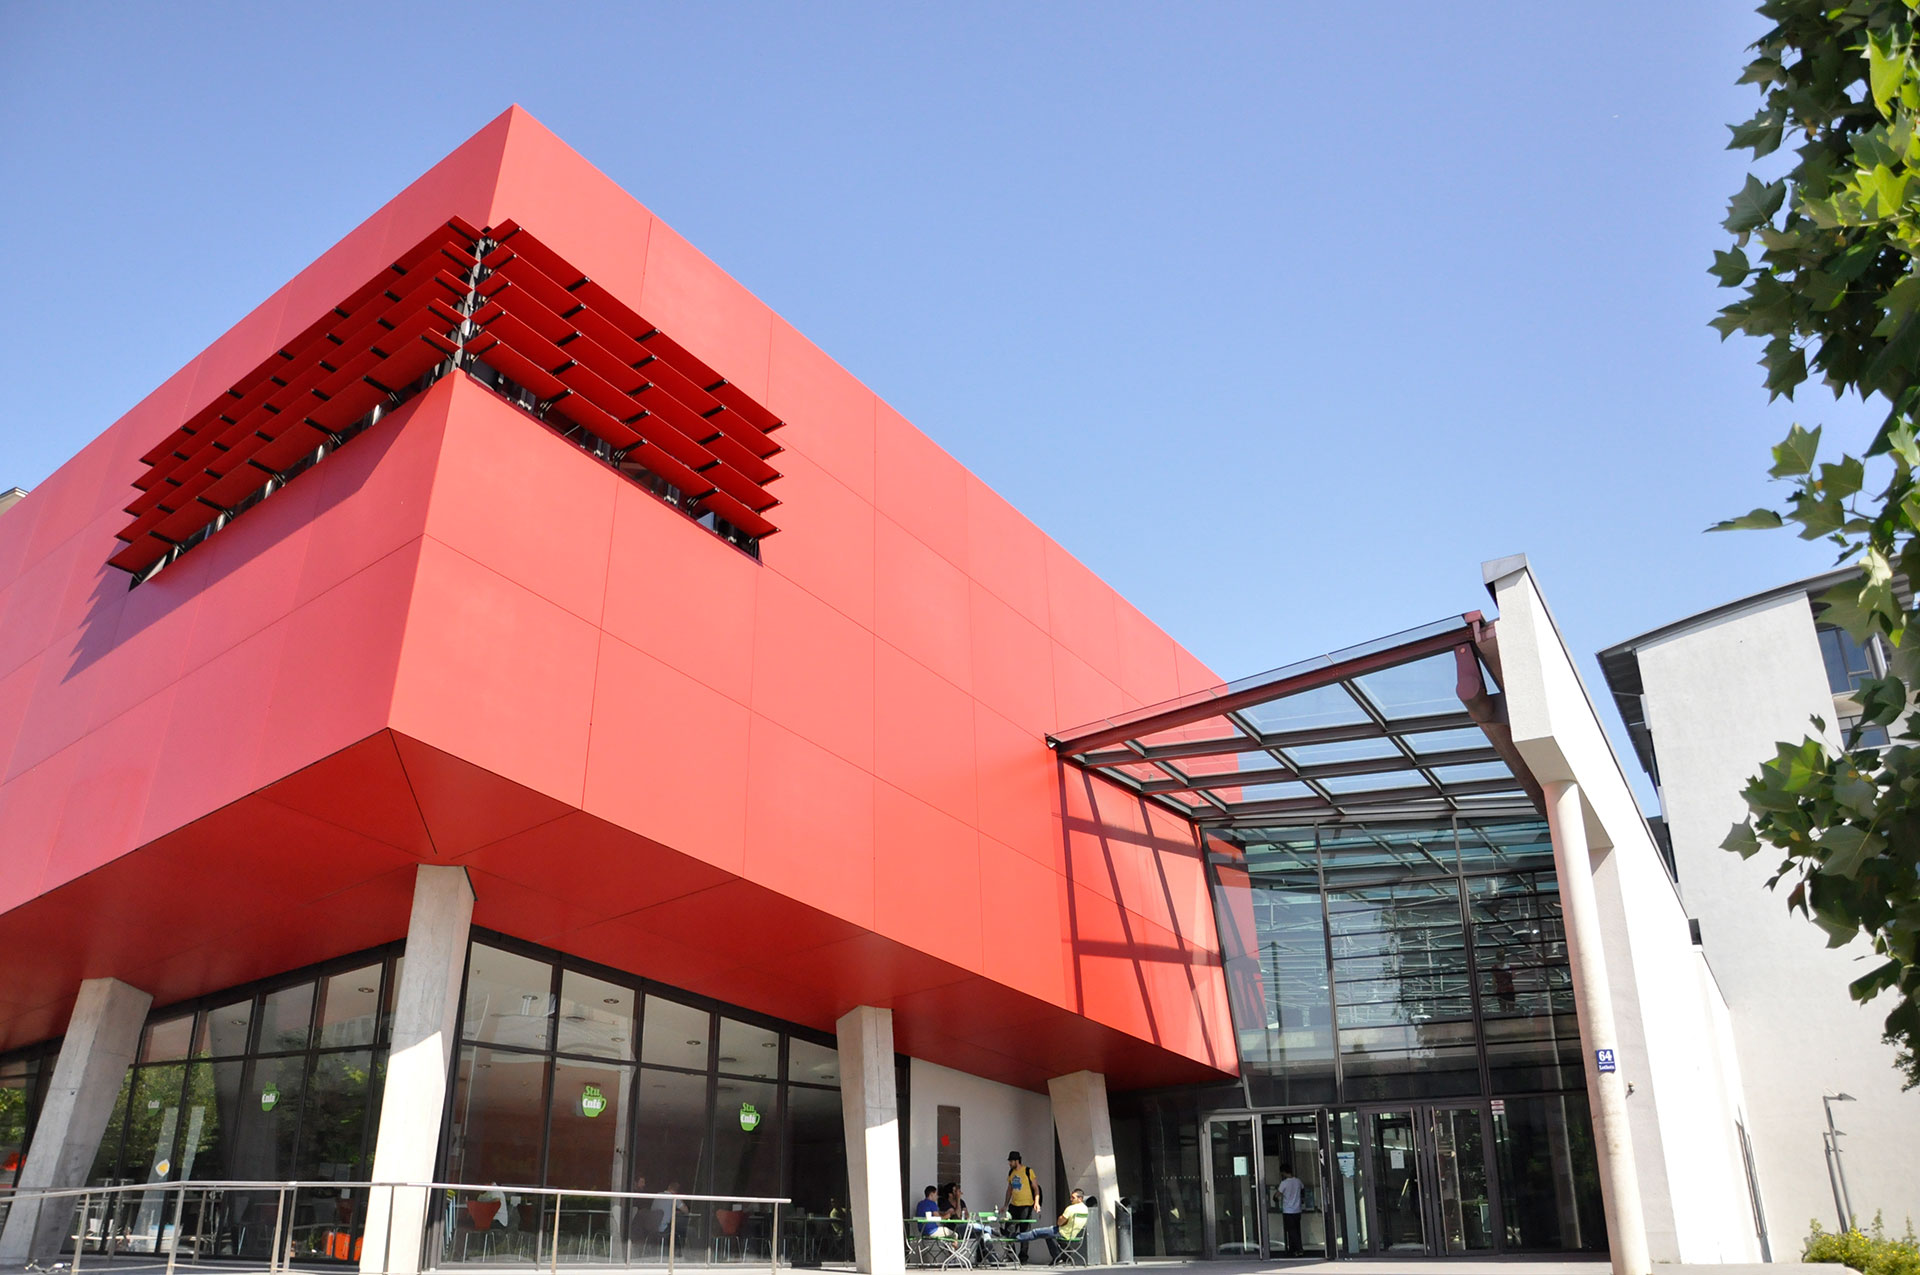
\includegraphics[width=\textwidth]{assets/dm_roter_wuerfel_ben_steinig.jpg}
      \caption{Symbolbild Projekt}
    \end{figure}
  \end{column}
\end{columns}
\end{frame}

\section{Blöcke und Boxen}
\begin{frame}{Verschiedene Blocktypen}
\begin{block}{Standardblock}
  Neutrale Information oder Definition
\end{block}

\begin{exampleblock}{Beispiel}
  Praktisches Anwendungsbeispiel
\end{exampleblock}

\begin{alertblock}{Wichtiger Hinweis}
  Warnung oder besonders wichtige Information
\end{alertblock}
\end{frame}

\begin{frame}{Block mit Liste}
\begin{block}{Erfolgsfaktoren}
  \begin{itemize}
    \item Klare Zielsetzung
    \item Engagiertes Team
    \item Regelmäßiges Monitoring
    \item Offene Kommunikation
  \end{itemize}
\end{block}
\end{frame}

\section{Mathematik und Formeln}
\begin{frame}{Formeln und Berechnungen}
Eine einfache Gleichung:
\[
E = mc^2
\]

\vspace{0.5cm}
Komplexere Berechnungen:
\[
f(x) = \int_{-\infty}^{\infty} e^{-x^2} \, dx = \sqrt{\pi}
\]

\vspace{0.3cm}
Inline-Mathematik: Die Lösung ist $x = \frac{-b \pm \sqrt{b^2-4ac}}{2a}$
\end{frame}

\section{Quellenangaben}
\begin{frame}{Quellen und Referenzen}
\small
\textbf{Literatur:}
\begin{itemize}
  \item Müller, A. (2024): \textit{Effektive Präsentationen}. München: Fachverlag.
  \item Schmidt, B. \& Weber, C. (2023): „Visuelle Kommunikation in der Wissenschaft". \textit{Journal of Communication}, 15(3), S. 234--256.
  \item Online-Quelle: \url{https://www.beispiel.de/artikel}
\end{itemize}
\end{frame}

% Zitierleitfaden folgt nach den allgemeinen Quellenangaben

\begin{frame}{Quellen und Referenzen}
\small
\textbf{Bildquellen:}
\begin{itemize}
  \item Abbildung 1: Eigene Darstellung
  \item Abbildung 2--4: Creative Commons Lizenz
\end{itemize}
\end{frame}

\section{Zitierleitfaden}
\begin{frame}{Zitierleitfaden: Sonderfälle (Beispiele)}
\small
\textbf{Kein Autor bekannt:}\\[2pt]
\textit{Geschichte des Internets.} (2023, 5. Mai). In \textit{Technologieportal.de}.\\
Abgerufen von \url{https://www.technologieportal.de/internet-geschichte}

\vspace{0.5\baselineskip}\hrule\vspace{0.5\baselineskip}

\textbf{Kein Veröffentlichungsdatum bekannt:}\\[2pt]
Wikipedia-Autoren. (o. D.). \textit{Zukunft der Robotik}. In \textit{Wikipedia – Die freie Enzyklopädie}.\\
Abgerufen von \url{https://de.wikipedia.org/wiki/Robotik}

\vspace{0.5\baselineskip}\hrule\vspace{0.5\baselineskip}

\textbf{Kein Titel vorhanden:}\\[2pt]
Bundesministerium für Bildung und Forschung. (2024). {[}Pressemitteilung über neue KI-Förderung{]}.\\
Abgerufen von \url{https://www.bmbf.de/ki-presse}

\end{frame}

% Split continuation of special cases onto a new frame to avoid cutoff
\begin{frame}{Zitierleitfaden: Sonderfälle (Beispiele)}
\small
\textbf{Kein Autor und kein Datum:}\\[2pt]
\textit{Digitalisierung im Alltag}. (o. D.). In \textit{TechWorld Online}.\\
Abgerufen von \url{https://www.techworld.de/digitalisierung}

\vspace{0.5\baselineskip}\hrule\vspace{0.5\baselineskip}

\textbf{Ganze Website statt einzelner Seiten:}\\[2pt]
Wikipedia. (o. D.). \textit{Wikipedia – Die freie Enzyklopädie}. \url{https://de.wikipedia.org}
\end{frame}

\begin{frame}{Zitierleitfaden: Zusammenfassung}
\small
\begin{table}
  \centering
  \begin{tabular}{>{\raggedright\arraybackslash}p{0.24\textwidth} >{\raggedright\arraybackslash}p{0.52\textwidth} >{\raggedright\arraybackslash}p{0.20\textwidth}}
    \toprule
    \textbf{Fall} & \textbf{Beispiel} & \textbf{Besonderheit} \\
    \midrule
    Kein Autor & \textit{Titel der Seite}. (2023). Website. URL & Titel an erster Stelle \\
    Kein Datum & Autor. (o. D.) & o. D. = ohne Datum \\
    Kein Titel & Autor. (2024). {[}Beschreibung{]}. Website. URL & Beschreibung in eckigen Klammern \\
    Kein Autor \& kein Datum & \textit{Titel}. (o. D.) Website. URL & Beides kombiniert \\
    Ganze Website & Organisation. (o. D.). Website-Name. URL & Kein Artikel nötig \\
    \bottomrule
  \end{tabular}
\end{table}
\end{frame}

\section{Literatur (biblatex)}
\begin{frame}{Zitieren im Text}
\small
\textbf{Beispiele:}
\begin{itemize}
  \item Narrative Zitation: \textcite{mueller2024} betont die Bedeutung klarer Struktur.
  \item Parenthetisch: Neuere Studien zeigen Vorteile \parencite{schmidt2023}.
  \item Online-Ressourcen eignen sich f\"ur Einstiege \parencite{beispielOnline}.
\end{itemize}
\end{frame}

\begin{frame}{Fu\ss{}noten-Zitat}
Im Flie\ss{}text mit vollst\"andiger Referenz in der Fu\ss{}note\footfullcite{mueller2024}.

\vspace{0.5\baselineskip}
Weitere Erw\"ahnungen k\"onnen k\"urzer erfolgen \parencite{mueller2024, schmidt2023}.
\end{frame}

\begin{frame}[allowframebreaks]{Literaturverzeichnis}
% In Beamer ohne zus\"atzliche \section-\"Uberschrift
\printbibliography[heading=none]
\end{frame}

\section{Zusammenfassung}
\begin{frame}{Zusammenfassung}
\begin{itemize}
  \item Fassen Sie die Kernaussagen zusammen und leiten Sie zu nächsten Schritten über.
  \item Nutzen Sie optional die Akzentfarbe \textcolor{HMRed}{HM-Rot} für Highlights.
  \item Schließen Sie mit einem klaren Call-to-Action oder einer Kontaktinformation.
\end{itemize}
\end{frame}

\begin{frame}[plain]
\begin{center}
  \vspace{2cm}
  {\Huge \textbf{Vielen Dank!}}
  
  \vspace{1cm}
  {\Large Fragen und Diskussion}
  
  \vspace{1.5cm}
  \textbf{Kontakt:}\\
  vorname.nachname@hm.edu
\end{center}
\end{frame}

\end{document}
